\documentclass[../Presentation.tex]{subfiles}
\usepackage[utf8]{inputenc}
\title{Estructura de Datos}
\subtitle{Estructura de Datos en C}
\author{José Everardo Torres O.}
\usetheme{lucid}
\begin{document}
\frame{
\titlepage
}
\frame{
\frametitle{Tabla Hash}
En los capitulos anteriores, hemos visto en varias tecnicas de busqueda. Considere un problema de busqueda en un arreglo. Si el arreglo no esta ordenado entonces no tendremos otra opcion que ver uno a uno los elementos, entonces el tiempo de complejidad seria \textbf{$O(n)$}. Si el arreglo esta ordenado, entonces podemos buscar el valor que queremos en tiempo $O(logn)$ tiempo logaritmico usando busqueda binaria.\\
\note{Las tablas de datos permiten el acceso directo a un elemento de una secuencia, indicando la posicion que ocupan.}
Pero ¿que si tenemos una función que puede brindarnos el indice/ubicación de el valor que estamos buscando en el arreglo?
}
\frame{
Nosotros podemos ir directamente a la ubicación y decirnos si nuestrbo objeto dentro de la busqueda esta presente o no en tiempo constante $O(1)$ . Esta función es llamada Hash.
\note{
 La potencia de las tablas hash o dispersas radica en la busqueda de elementos ya que conociendo el campo clave, se puede obtener directamente la posición que ocupa, y por consiguiente la información asociada con dicha clave.}
El estudio de tablas hash acarrea el estudio de funciones hash o dispersión, que mediante expresiones matemaicas permiten obtener direcciones segun una clave que es el argumento de la función.
}
\frame{
Por lo tanto: \textbf{Tabla Hash} es una estructura de datos, que asigna claves a valores. Cada posición de las Tablas Hash es llamada un espacio(slot). La tabla hash usa una función has para calcular el indice de un  arreglo de espacios. Usamos la tabla hash cuando el número de claves realmente almacenadas es pequeño para el número de claves posibles.
\begin{figure}
	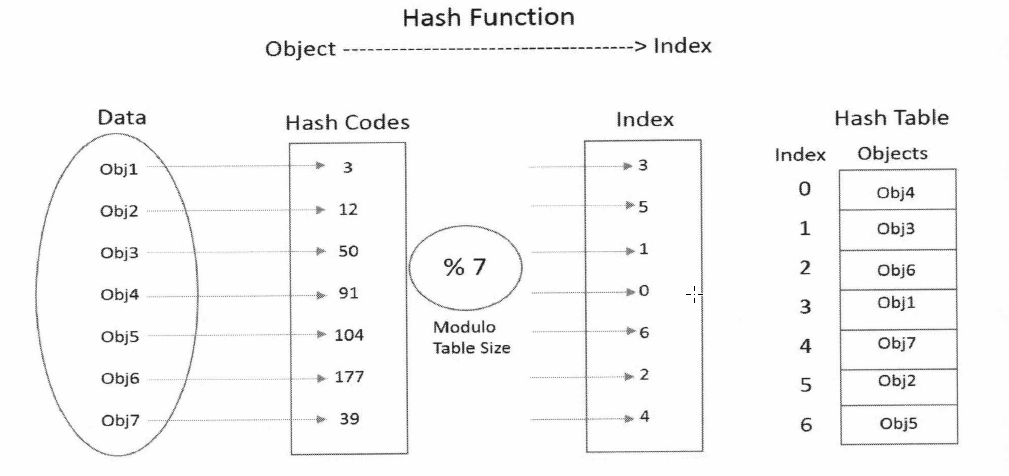
\includegraphics[scale=0.5]{Hash Table Example}
	\caption{\label{fig:TableHashExample} Ejemplo de una Tabla Hash}
\end{figure}
}
\end{document}